%
% lissajous.tex -- Lissajous figure
%
% (c) 2020 Prof Dr Andreas Müller, Hochschule Rapperswil
%
\documentclass[tikz,12pt]{standalone}
\usepackage{times}
\usepackage{amsmath}
\usepackage{txfonts}
\usepackage[utf8]{inputenc}
\usepackage{graphics}
\usepackage{color}
\usepackage{pifont}
\usetikzlibrary{arrows,intersections,math,calc}
\begin{document}

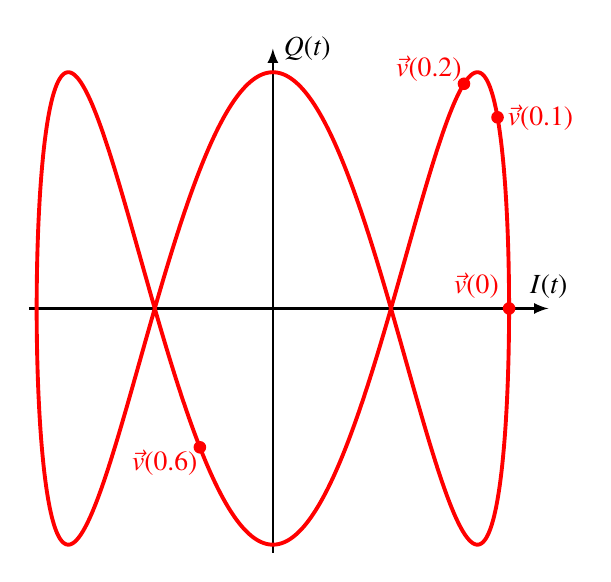
\begin{tikzpicture}[>=latex,thick]

\draw[->] (-3.1,0)--(3.5,0) coordinate[label={$I(t)$}];
\draw[->] (0,-3.1)--(0,3.3) coordinate[label={right:$Q(t)$}];

\draw[color=red,line width=1.4pt]
	plot[domain=0:2,samples=1000]
		({3*cos(\x*180)},{3*sin(3*\x*180)});

\foreach \x in {0,0.1,0.2,0.6}{
	\fill[color=red] ({3*cos(\x*180)},{3*sin(3*\x*180)})
		circle[radius=0.08];
}

\node[color=red] at (3,0) [above left] {$\vec{v}(0)$};

\node[color=red] at ({3*cos(0.1*180)},{3*sin(3*0.1*180)})
	[right] {$\vec{v}(0.1)$};

\node[color=red] at ({3*cos(0.2*180)+0.1},{3*sin(3*0.2*180)-0.1})
	[above left] {$\vec{v}(0.2)$};

\node[color=red] at ({3*cos(0.6*180)+0.1},{3*sin(3*0.6*180)+0.1})
	[below left] {$\vec{v}(0.6)$};

\end{tikzpicture}

\end{document}

